Thermal systems are typically characterized by macroscopic quantities — temperature, pressure, and volume — that arise from the statistical behavior of an enormous number of microscopic constituents. Each molecule in a gas, for example, possesses a definite position and velocity at every instant, but these details are not individually tracked; instead, macroscopic observables summarize the collective dynamics of trillions of particles.

A single macroscopic state can correspond to an enormous number of microscopic configurations. The same pressure and temperature in a gas can arise from countless different combinations of individual molecular positions and velocities. This multiplicity is central to statistical mechanics, where a macroscopic description averages over the detailed microstates that realize it.

Entropy quantifies the logarithm of the number of microstates compatible with a given macrostate. In the Boltzmann formulation, the entropy $S$ of a system is expressed as $S = k_B \ln \Omega$, where $k_B$ is Boltzmann's constant and $\Omega$ denotes the number of microstates. This mathematical structure captures both the multiplicity of configurations and the incompleteness of macroscopic information.

The second law of thermodynamics asserts that in an isolated system, entropy cannot decrease. Natural processes tend toward macrostates with greater multiplicity because they are overwhelmingly more probable. The law governs the irreversibility observed in macroscopic phenomena and forbids spontaneous reorganization into low-entropy configurations without external intervention.


Over time, systems evolve toward equilibrium configurations not by deterministic rearrangement, but through overwhelmingly probable statistical tendencies. The microscopic dynamics may allow rare fluctuations into low-entropy states, yet the vast majority of accessible microstates correspond to thermal equilibrium, ensuring that systems overwhelmingly move toward higher entropy.

The second law of thermodynamics admits multiple equivalent formulations. In the Clausius statement, it forbids the spontaneous flow of heat from a colder body to a hotter one. In the Kelvin statement, it rules out the complete conversion of heat into mechanical work in a cyclic process without any other effect. Both formulations capture the unidirectional dispersal of energy and the impossibility of constructing perpetual motion machines of the second kind.

While the underlying microscopic laws — Newtonian mechanics or the Schrödinger equation — are time-reversal invariant, macroscopic irreversibility emerges from statistical asymmetry. Individual molecular collisions remain reversible, but the aggregate behavior overwhelmingly favors transitions toward higher-entropy macrostates due to the vast numerical dominance of such configurations.

Although the total phase space volume occupied by a system is conserved under Hamiltonian evolution, as guaranteed by Liouville's theorem, entropy can nonetheless increase. Fine-grained distributions evolve into increasingly intricate structures that, when viewed with any coarse-graining appropriate to macroscopic observations, appear progressively more uniform, thus corresponding to higher entropy.

Temperature reflects the average kinetic energy per degree of freedom in a system. In classical gases, the distribution of particle energies follows the Maxwell–Boltzmann distribution, while in more general statistical ensembles, the Boltzmann distribution governs the probability of finding the system in a given microstate, establishing a precise link between microscopic motion and macroscopic thermodynamic parameters.

Thermodynamic processes exchange energy between systems through work and heat, but entropy tracks the irreversible dispersal of energy and the loss of access to precise microscopic configurations. While work represents organized energy transfer and heat denotes disorganized exchange, the second law constrains their interplay, ensuring that some fraction of energy always becomes unavailable for doing work.

The second law introduces a preferred temporal direction, often termed the thermodynamic arrow of time. This arrow is not derived from the fundamental laws of motion, which are time-symmetric, but from the statistical tendency toward higher entropy. As entropy increases, systems evolve from ordered to disordered states, establishing an emergent asymmetry between past and future.

The increase of entropy is not a mechanistic necessity imposed by the microscopic equations of motion, but a near certainty based on phase space volumes. The number of microstates corresponding to high-entropy macrostates so vastly exceeds those of low-entropy macrostates that, although a reversal is technically possible, it is statistically negligible on any practical timescale.

The rise of entropy presumes a process of coarse-graining — grouping together microscopic configurations that are indistinguishable at the macroscopic level. Fine-grained correlations and fluctuations, though preserved in principle by microscopic dynamics, become irrelevant for macroscopic observables, allowing entropy to increase from the observer's practical standpoint.

Entropy can thus be reinterpreted as missing information about the system's precise microstate. In this view, thermodynamic entropy parallels concepts from information theory, linking the physical evolution of systems with the epistemic limitations inherent in macroscopic descriptions.

In 1867, James Clerk Maxwell introduced a thought experiment that challenged the apparent absoluteness of the second law of thermodynamics. He imagined a sealed box filled with gas at thermal equilibrium, where molecules moved randomly at a range of speeds and directions. A partition divided the box into two chambers, A and B, with a small frictionless door controlled by a hypothetical observer — the demon.

The demon's intervention does not involve the input of mechanical work or external energy. Instead, it passively monitors individual molecules approaching the door. When a fast-moving molecule from chamber A nears the door, the demon opens it, allowing the molecule into chamber B. When a slow-moving molecule from B approaches, it is allowed into chamber A. Molecules not meeting these criteria are blocked. Over time, faster molecules accumulate in B, and slower ones in A.

\begin{center}
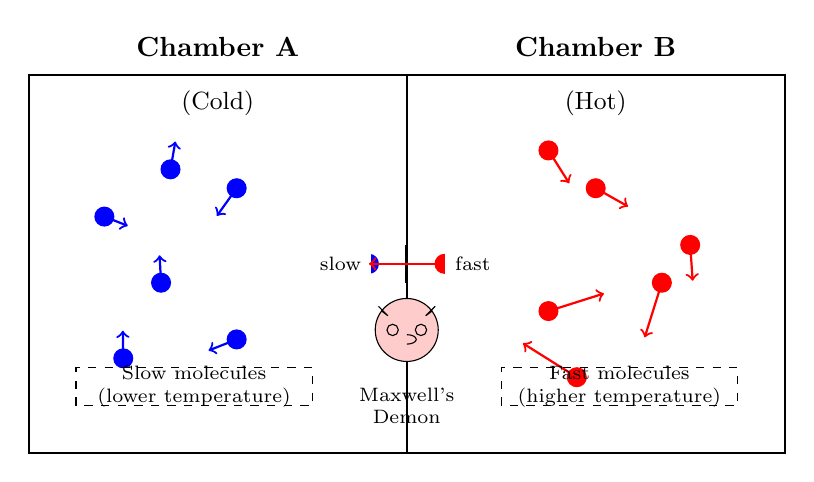
\begin{tikzpicture}[scale=1.2]
    \draw[thick] (0,0) rectangle (8,4);
    \draw[thick] (4,0) -- (4,4);
    \node[font=\bfseries] at (2,4.3) {Chamber A};
    \node[font=\bfseries] at (6,4.3) {Chamber B};
    \node[font=\small] at (2,3.7) {(Cold)};
    \node[font=\small] at (6,3.7) {(Hot)};
    \draw[very thick, fill=black!10] (4,1.8) -- (4,2.2);
    \node[draw, circle, fill=red!20, minimum size=0.8cm] (demon) at (4,1.3) {};
    \draw (demon) -- ++(0.2,0.15) -- ++(0.1,0.1);
    \draw (demon) -- ++(-0.2,0.15) -- ++(-0.1,0.1);
    \draw (demon) -- ++(0,0.4);
    \draw (demon.center) ++(0.15,0) circle (0.06);
    \draw (demon.center) ++(-0.15,0) circle (0.06);
    \draw (demon.center) ++(0,-0.15) arc (270:450:0.1 and 0.05);
    \foreach \x/\y in {1.0/1.0, 0.8/2.5, 1.5/3.0, 2.2/1.2, 2.2/2.8, 1.4/1.8}{
        \draw[thick, blue, ->] (\x,\y) -- ++({0.3*cos(rnd*360)},{0.3*sin(rnd*360)});
        \filldraw[blue] (\x,\y) circle (0.1);
    }
    \foreach \x/\y in {5.5/1.5, 6.0/2.8, 5.5/3.2, 6.7/1.8, 7.0/2.2, 5.8/0.8}{
        \draw[thick, red, ->] (\x,\y) -- ++({0.6*cos(rnd*360)},{0.6*sin(rnd*360)});
        \filldraw[red] (\x,\y) circle (0.1);
    }
    \filldraw[blue] (3.6,2.0) circle (0.1);
    \draw[->, thick, blue] (3.6,2.0) -- (4.4,2.0);
    \node[draw=white, fill=white, font=\scriptsize] at (3.3,2.0) {slow};
    \filldraw[red] (4.4,2.0) circle (0.1);
    \draw[->, thick, red] (4.4,2.0) -- (3.6,2.0);
    \node[draw=white, fill=white, font=\scriptsize] at (4.7,2.0) {fast};
    \draw[dashed] (0.5,0.5) rectangle (3.0,0.9);
    \node[align=center, font=\scriptsize] at (1.75,0.7) {Slow molecules\\(lower temperature)};
    \draw[dashed] (5.0,0.5) rectangle (7.5,0.9);
    \node[align=center, font=\scriptsize] at (6.25,0.7) {Fast molecules\\(higher temperature)};
    \node[align=center, font=\scriptsize] at (4,0.5) {Maxwell's\\Demon};
\end{tikzpicture}
\end{center}

This selective sorting induces a temperature gradient where none previously existed. Heat flows from the colder to the hotter chamber without any external energy input, in direct contradiction to the Clausius formulation of the second law. From a statistical standpoint, entropy appears to decrease: the initially uniform, high-entropy configuration is replaced by a more ordered state characterized by a temperature difference.

The paradox arises because no mechanical work is performed and no external energy is introduced, yet the system evolves toward a lower-entropy configuration. The demon, by choosing which molecules to admit or block, seems capable of circumventing the thermodynamic constraints that govern ordinary processes.

Modern resolutions of the paradox reinterpret the demon not as an idealized observer, but as a physical system subject to thermodynamic limitations. To make decisions, the demon must measure molecular properties and store the resulting information in a memory structure that is itself embodied in matter.

Information, however, is not abstract — it is physical. In 1961, Rolf Landauer demonstrated that erasing one bit of information requires a minimum energy dissipation of $k_B T \ln 2$, where $k_B$ is Boltzmann's constant and $T$ the temperature of the environment. Erasure generates heat and increases the entropy of the surroundings, preserving the second law.

Building on Landauer's insight, Charles Bennett showed that the entropy cost of erasing the demon's memory cancels the entropy reduction achieved by sorting molecules. Thus, while the demon temporarily lowers entropy in the gas, it ultimately pays the required thermodynamic cost through information erasure.

Yet this resolution raises deeper questions. The energy cost is associated not with sorting the molecules, but with processing and erasing information. This suggests that irreversibility is linked not only to energy flows but also to logical operations, redefining the connection between information theory and thermodynamics.

Further scrutiny probes the assumptions involved. Is erasure truly the only thermodynamically costly step? Can measurements be performed without disturbing the system? If information is preserved indefinitely without erasure, does the paradox remain unresolved?

Quantum mechanics intensifies these challenges. In quantum systems, measurement necessarily perturbs the state being observed, and particles obey indistinguishability and entanglement rules that constrain sorting operations. The demon paradox thus resurfaces in quantum contexts, illuminating the intricate ties among thermodynamics, information, and the structure of physical law.

\begin{SideNotePage}{
  \textbf{Maxwell's Demon and Information Thermodynamics:} \par
  This illustration depicts James Clerk Maxwell's famous thought experiment challenging the second law of thermodynamics. The top section shows the demon's operation: a hypothetical entity controls a frictionless door between two chambers, selectively allowing fast-moving molecules into one side and slow-moving molecules into the other. Over time, this creates a temperature gradient from an initially uniform system without apparent energy input. The middle section demonstrates the paradox: the demon seems to decrease entropy (increase order) by sorting molecules, violating the principle that entropy must increase in isolated systems. The bottom section reveals the resolution: the demon must measure molecular velocities and store this information in memory. Landauer's principle shows that erasing one bit of information requires minimum energy dissipation of kBT ln 2, generating heat and increasing entropy in the environment. The entropy cost of information processing ultimately preserves the second law, linking thermodynamics to computation and revealing the physical nature of information itself.
}{45_MaxwellDemon/UNPOP SCI - MAXWELLS DEMON - vF.pdf}
\end{SideNotePage}

